\documentclass{revtex4-2}%
\usepackage[T1]{fontenc}%
\usepackage[utf8]{inputenc}%
\usepackage{lmodern}%
\usepackage{textcomp}%
\usepackage{lastpage}%
\usepackage{graphicx}%
%
%
%
\begin{document}%
\normalsize%


\begin{figure}[h!]%
\centering%
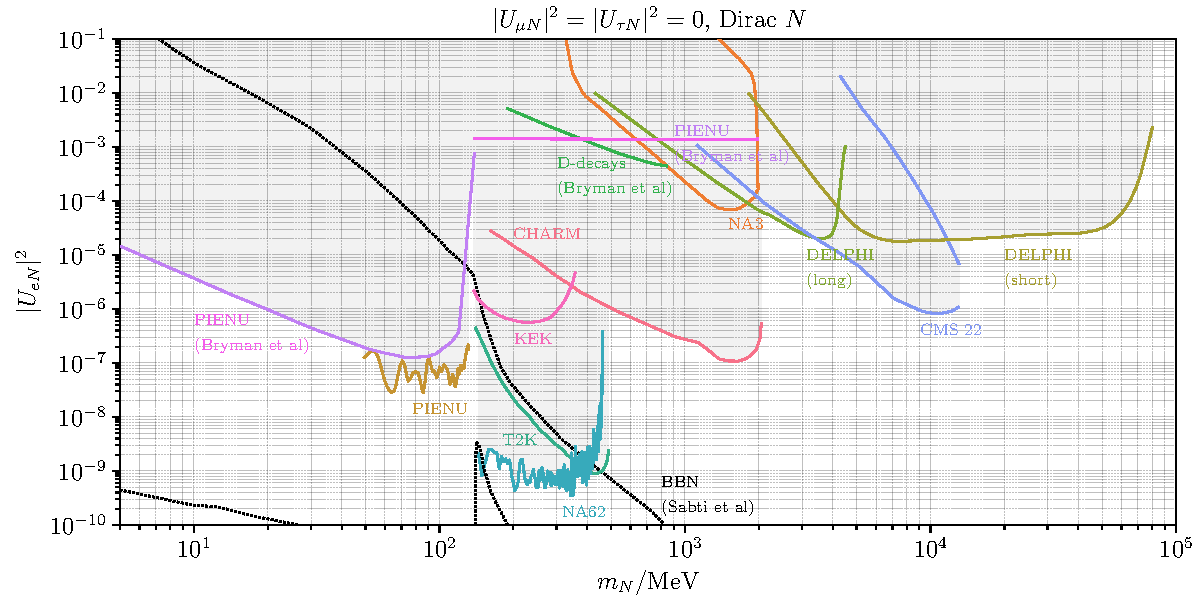
\includegraphics[width=1\textwidth]{../plots/UeN.pdf}%
\caption{Constraints on $C_{\rm{HN}\ell}^{e}/\Lambda^2 ~(\rm{GeV}^{-2})$ as a function of the HNL mass $m_N$. Limits shown: ATLAS (2019)~\cite{ATLAS:2019kpx}, ATLAS (2022)~\cite{ATLAS:2022atq}, BEBC(Barouki et al)~\cite{Barouki:2022bkt}, Belle~\cite{Belle:2013ytx}, Borexino~\cite{Borexino:2013bot}, CHARM~\cite{CHARM:1985nku}, CMS (2018)~\cite{CMS:2018iaf}, CMS (2022)~\cite{CMS:2022fut}, KENU (Bryman et al)~\cite{Bryman:2019bjg}, NA62~\cite{NA62:2020mcv}, PIENU (2017)~\cite{PIENU:2017wbj}, PIENU (Bryman et al)~\cite{Bryman:2019bjg}, PMNS Unitarity~\cite{Work in progress}, T2K~\cite{T2K:2019jwa}, TRIUMF~\cite{Britton:1992xv}.}%
\end{figure}

%


\begin{figure}[h!]%
\centering%
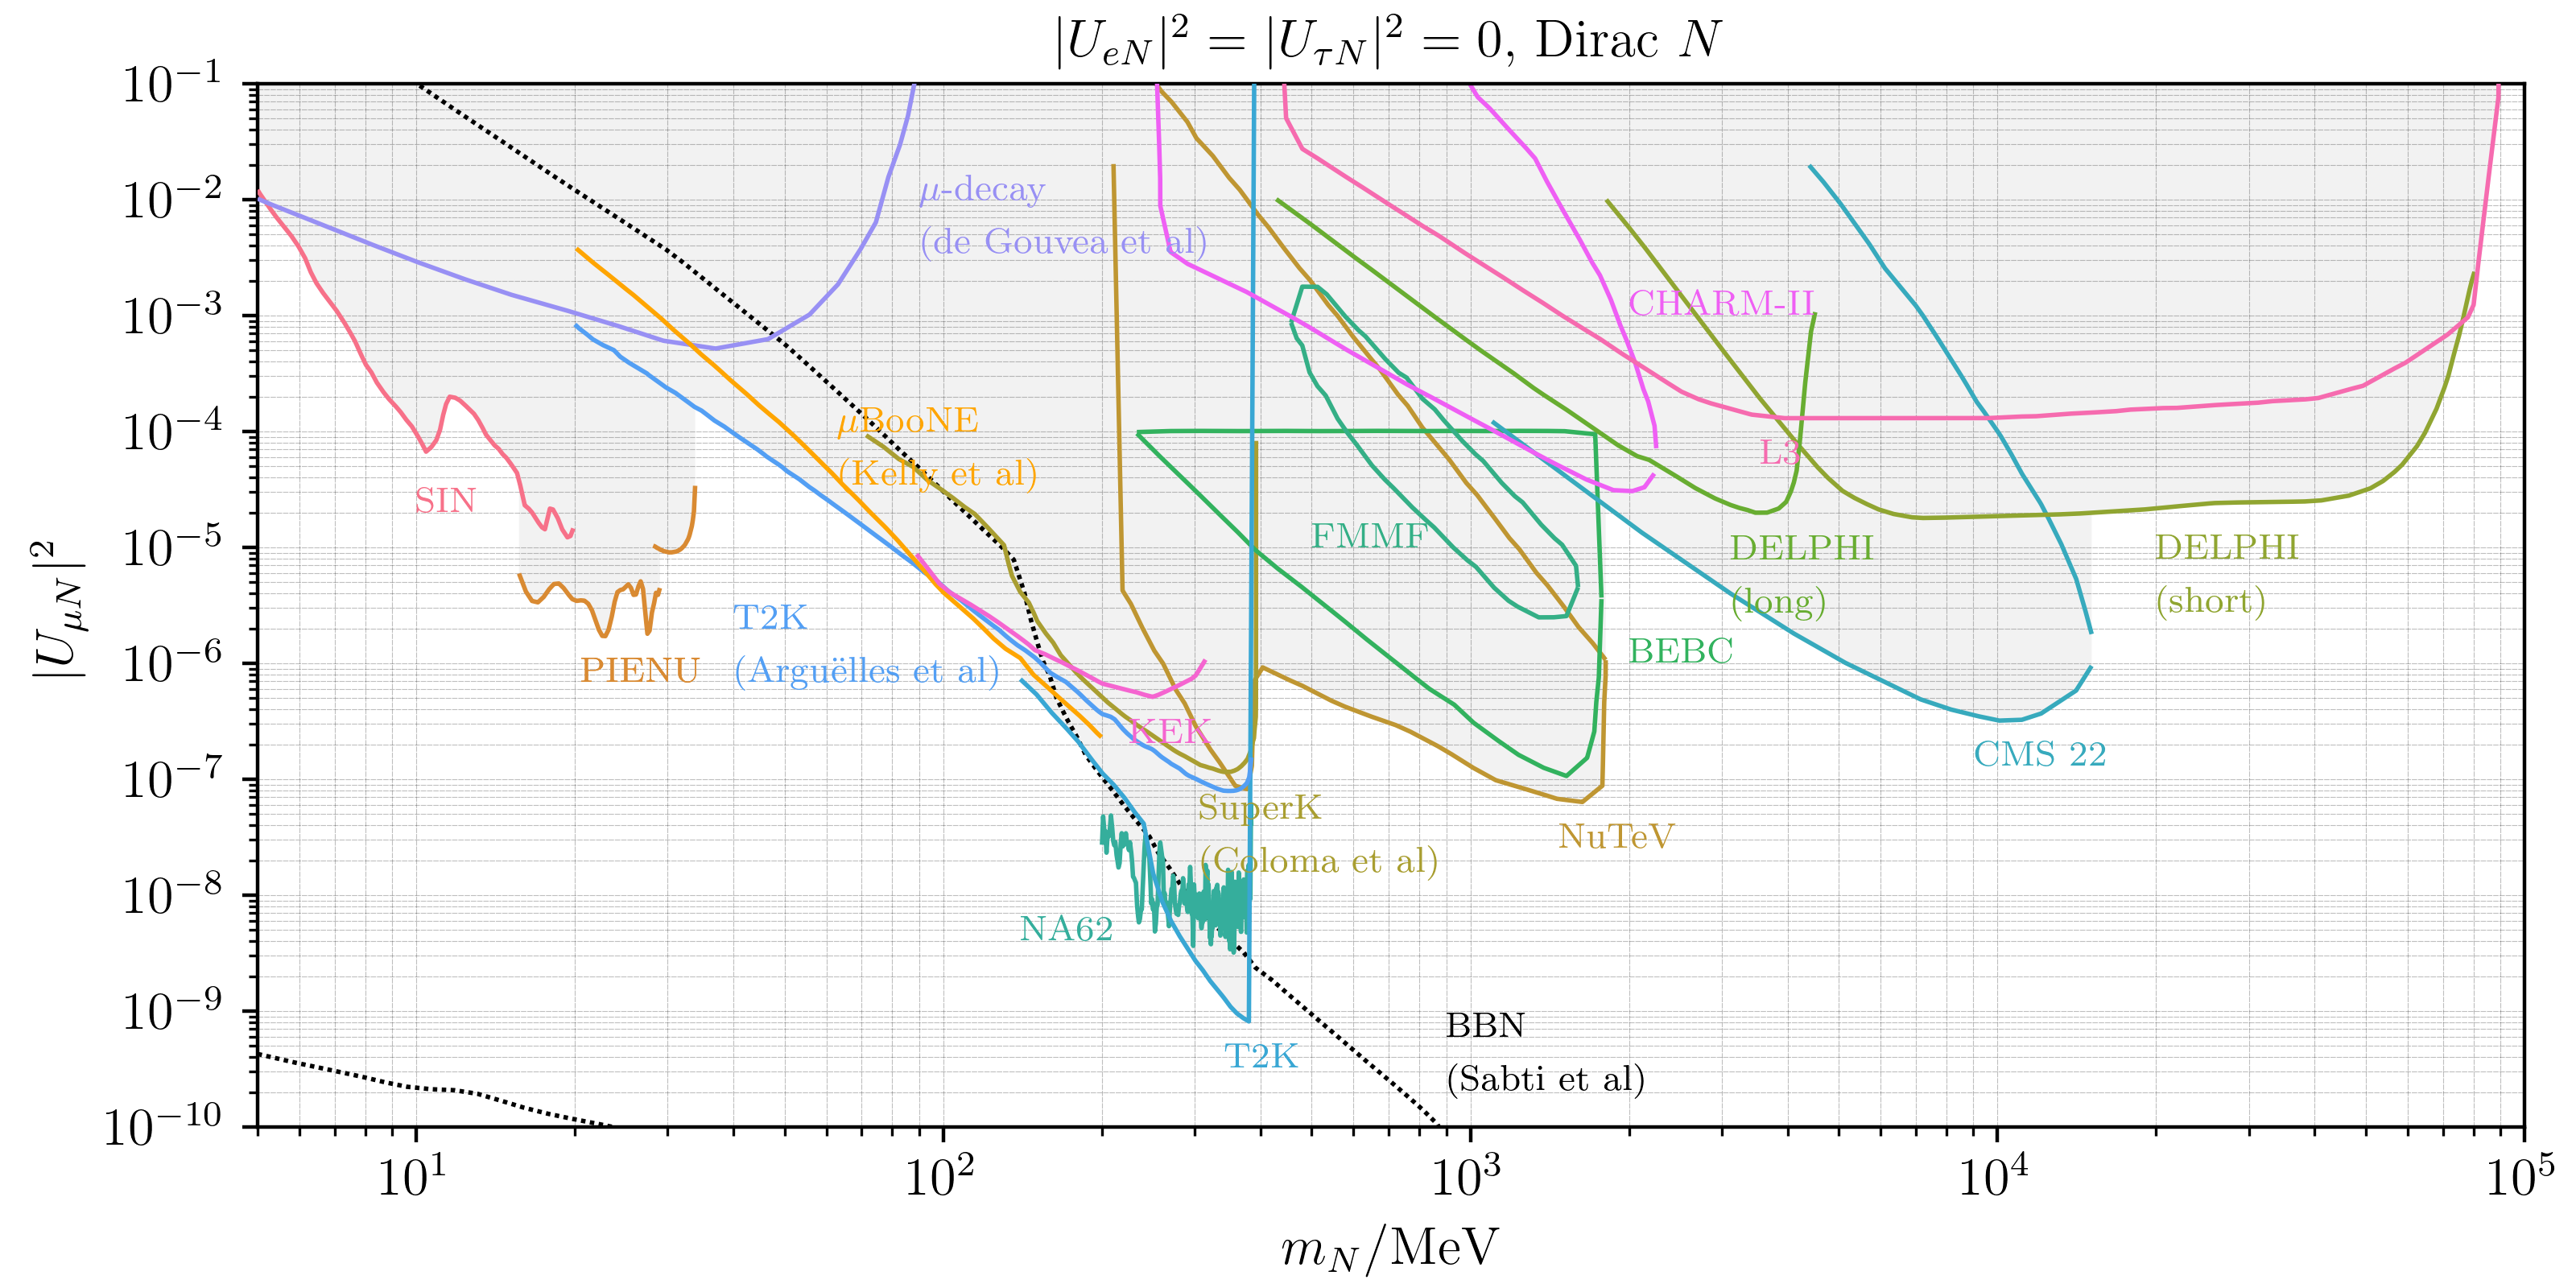
\includegraphics[width=1\textwidth]{../plots/UmuN.pdf}%
\caption{Constraints on $C_{\rm{HN}\ell}^{\mu}/\Lambda^2 ~(\rm{GeV}^{-2})$ as a function of the HNL mass $m_N$. Limits shown: $\mu$BooNE (Kelly et al)~\cite{Kelly:2021xbv}, $\mu\to N e \nu_e$~\cite{ParticleDataGroup:2022pth}, ATLAS (2019)~\cite{ATLAS:2019kpx}, ATLAS (2022)~\cite{ATLAS:2022atq}, BEBC~\cite{WA66:1985mfx}, CMS (2018)~\cite{CMS:2018iaf}, CMS (2022)~\cite{CMS:2022fut}, KEK~\cite{Bryman:2019bjg}, NA3~\cite{NA3:1986ahv}, NA62~\cite{NA62:2021bji}, NuTeV~\cite{NuTeV:1999kej}, PIENU~\cite{PIENU:2019usb}, PIENU(low $\mu$ energy)~\cite{PIENU:2019usb}, PMNS Unitarity~\cite{Work in progress}, PSI~\cite{Daum:1987bg}, T2K~\cite{T2K:2019jwa}, T2K (Arg\"uelles et al)~\cite{Arguelles:2021dqn}.}%
\end{figure}

%


\begin{figure}[h!]%
\centering%
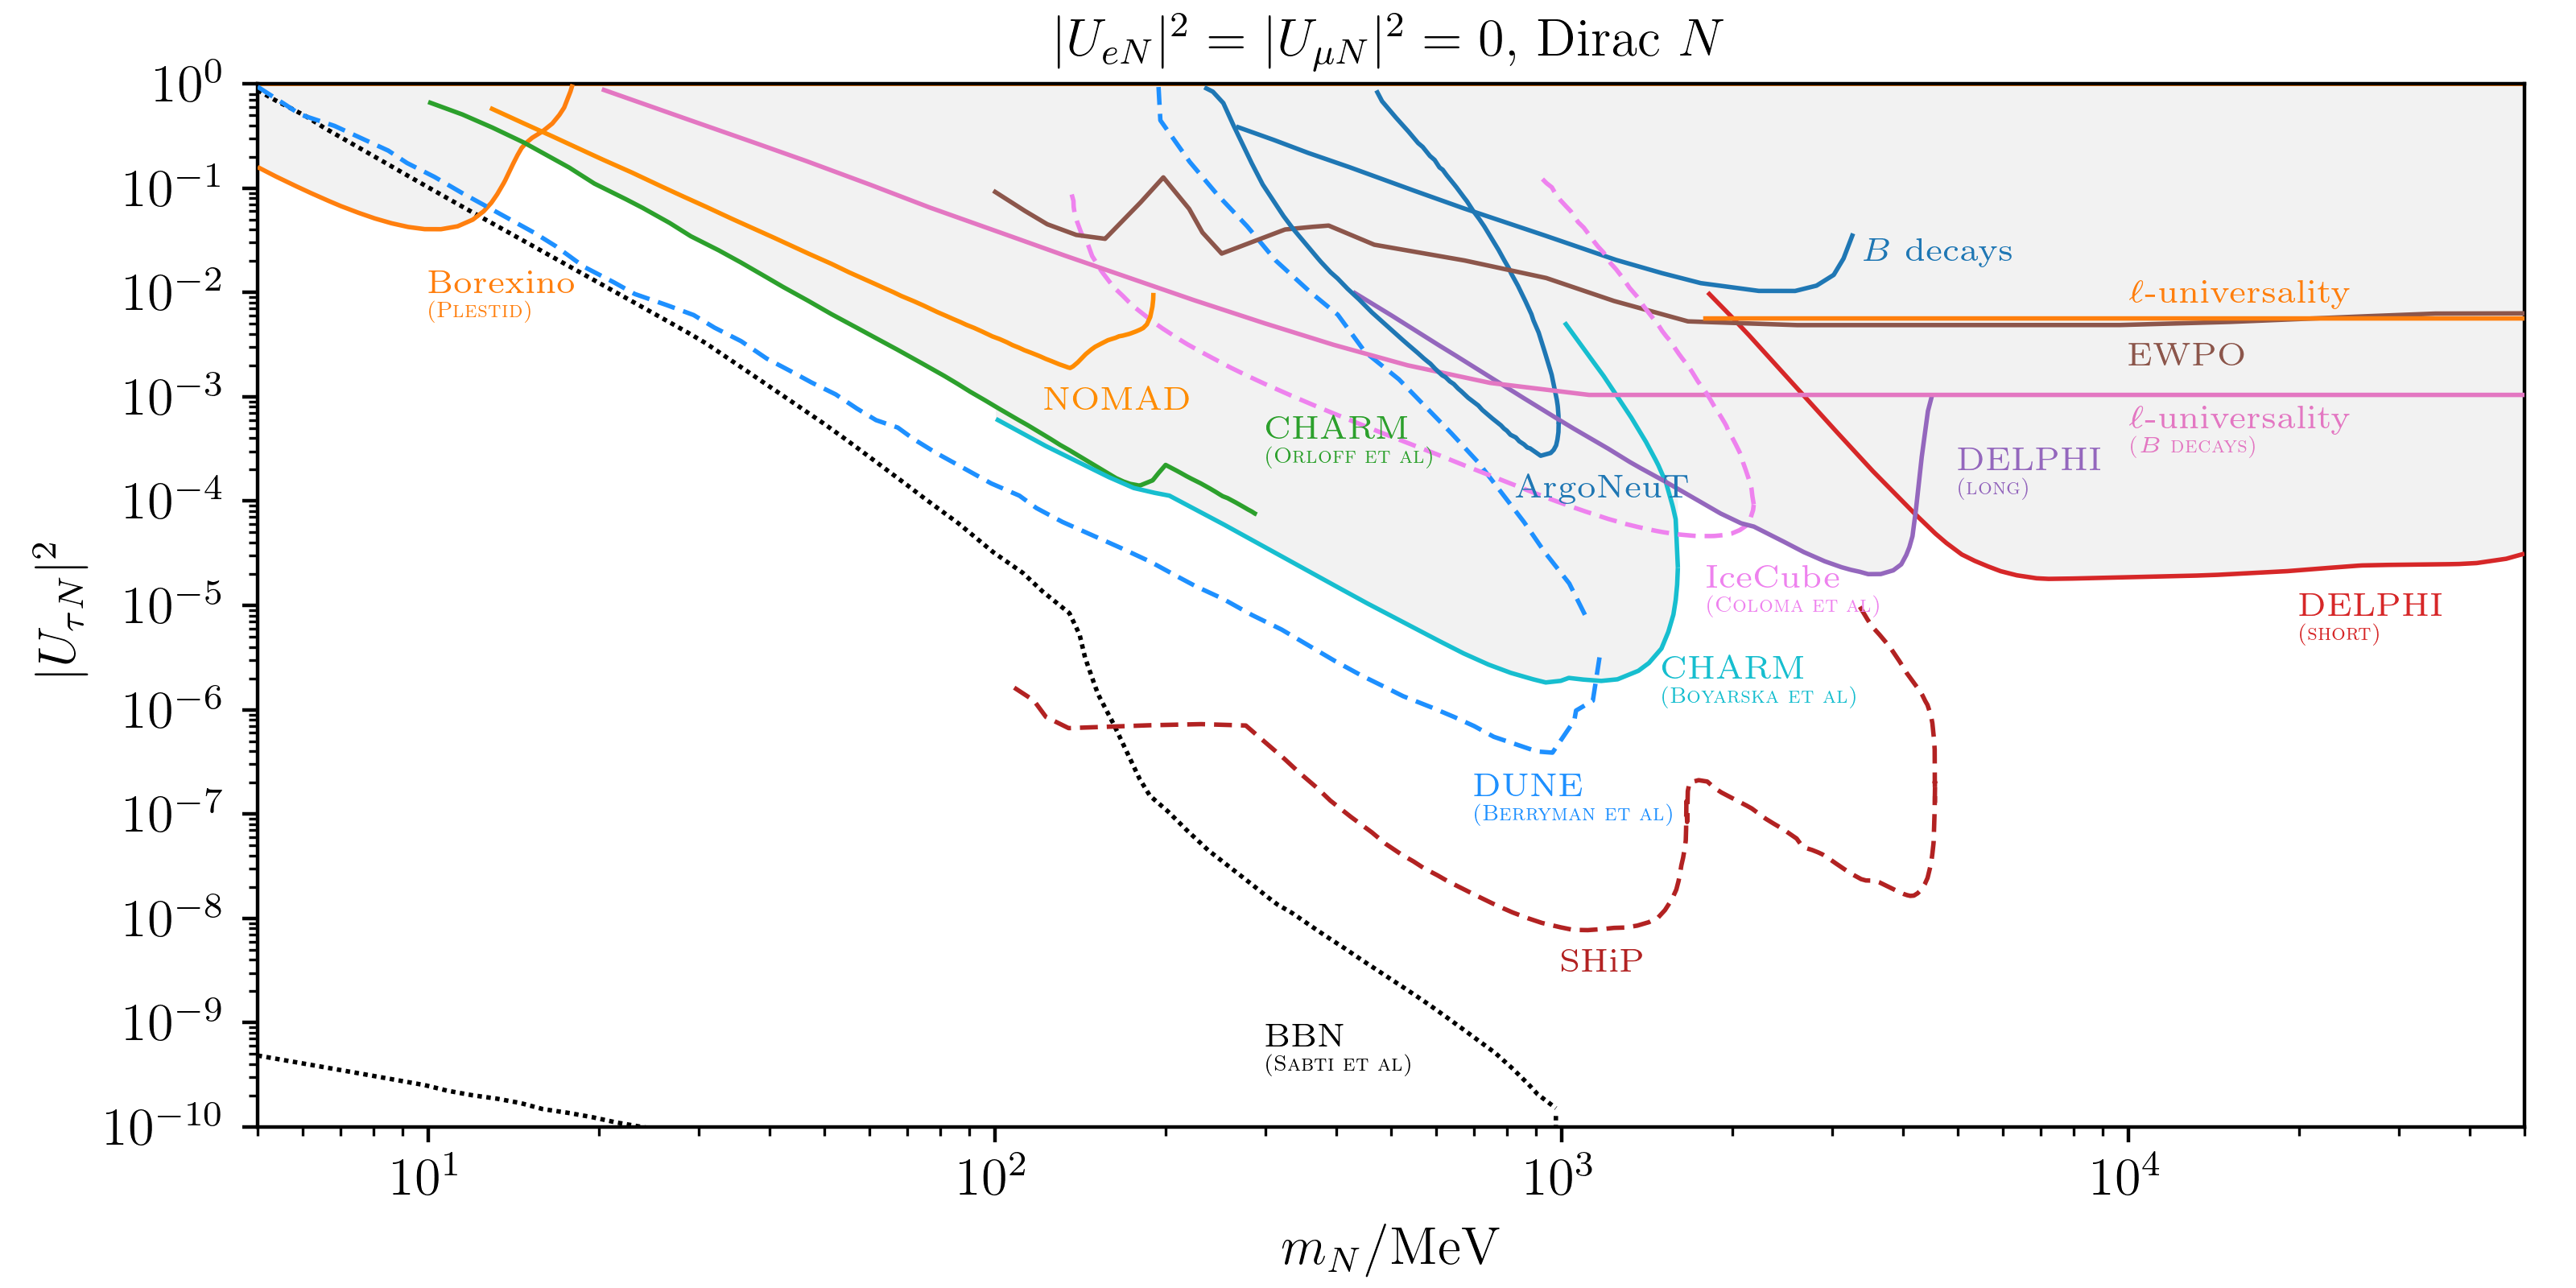
\includegraphics[width=1\textwidth]{../plots/UtauN.pdf}%
\caption{Constraints on $C_{\rm{HN}\ell}^{\tau}/\Lambda^2 ~(\rm{GeV}^{-2})$ as a function of the HNL mass $m_N$. Limits shown: $B\to N\tau$~\cite{ParticleDataGroup:2022pth}, $D\to N\tau$~\cite{ParticleDataGroup:2022pth}, $D_s\to N\tau$~\cite{ParticleDataGroup:2022pth}, $\tau\to N \mu \nu_\mu$~\cite{ParticleDataGroup:2022pth}, $\tau\to N e \nu_e$~\cite{ParticleDataGroup:2022pth}, PMNS Unitarity~\cite{Work in progress}.}%
\end{figure}

%
\bibliographystyle{apsrev4-1}%
\bibliography{bosonicCC_plots}%
\end{document}